\chapter{Bullseye: A parallel targeted facet imager}
\section{Design objectives}
The primary design objectives of this work is to build a scalable parallel facet-based imager. A full deconvolution pipeline is currently out of scope, instead 
the focus is on accelerating the gridding step, since this step will be called on multiple times in a major-minor cycle deconvolution pipeline as discussed in 
chapter \ref{chapter_synthesis}. To this end we will focus on comparing performance between parallel CPU-based resampling and a GPU approach.

\section{Architecture}
We've decided to split up the our implementation into two major components:
\begin{enumerate}
 \item A front-end program dealing with the logic of reading in measurement data, dealing with user options, overall program flow and image finalization.
 \item A set of back-end libraries that implement a common interface and house the resampling and transformation routines. The resampling routines include options to resample multiple
 correlations and enable faceting and w-projection logic.
\end{enumerate}

The architecture above allows us to easily swap out one set of resampling routines for another and to compare between CPU and GPU-based implementations. Figure~\ref{fig_arch} shows
the major components of our imager, along with several major dependencies. 
\begin{figure}[h]
  \begin{mdframed}
    \centering
    \begin{subfigure}[b]{0.66\textwidth}
      \centering
      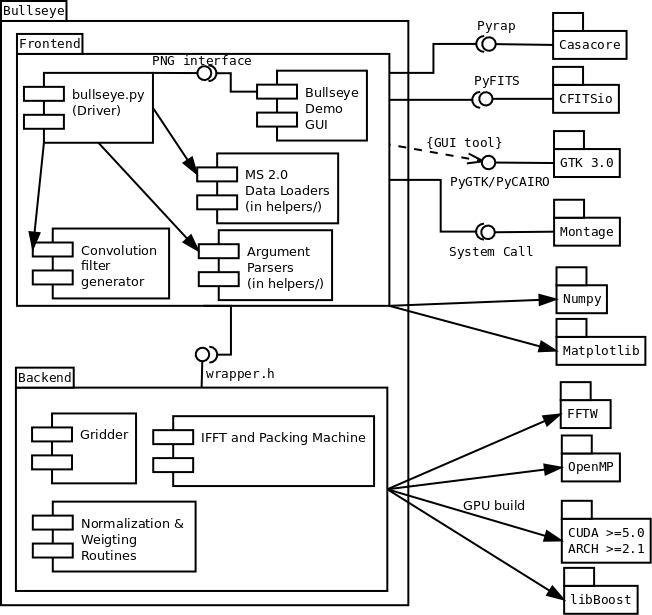
\includegraphics[width=\textwidth]{images/bullseye_arch.png}
      \caption{}
    \end{subfigure}  
    \caption[Bullseye Architecture]{The front end of the solution contains a commandline utility that has very similar options to that provided in other imagers, such as lwimager.
    Included with it are modules required to generate the w-projection convolution functions and a prototype graphical interface illustrating targeted faceting. The backend consists
    of the resampling routines along with routines to do fourier shifting, inversion and normalization on a set of facets that may each contain multiple spectral images.}
    \label{fig_arch}
  \end{mdframed}
\end{figure}

\section{Implementation strategy}
We opted to implement the front end of the program using Python 2.7 due to the the ease of implementing reading Measurement Sets, user option parsing and writing to Fits files provided by the python language and
the extension packages widely used within the radio astronomy community. The backend libraries containing the resampling routines has to be implemented in C++ to be efficient and have a common ctypes interface 
that can be called from Python. We opted to implement the backend libraries using constructs from the C++ 11 standard. The libraries contain a set of
templates shared between Cuda and CPU code to implement the resampling routines for the various use cases of the imager. Both the CPU and GPU code therefore
has to be compiled with the Nvidia NVCC compiler (versions 5.0 or above) toolkit.

\section{Normal workflow}
During imaging the user will supply a set of facet centre coordinates or number of facets splitting the sky (or both), along with a measurements database and outputs a set of facet images that can optionally
be recombined with the astronomical mosaicking package, Montage \cite{jacob2004montage}.

Program flow is indicated in Figure~\ref{fig_workflow}. The resampling and fourier inversion step may include sampling and transforming the sampling function.
The latter requires that all measurements are set to unity and a PSF is synthesized for each facet image. Additionally 
each facet may have resampling grids allocated for multiple correlations and spectral bands, and can therefore be facet cubes 
instead of simple 2D images. 

The fourier inversion step also entails shifting each of the facet grids such that the base uv-frequency of each grid
is located in the middle of the grids, thus shifting the image phase centre to the middle of each of the images.
\begin{figure}[ht!]
 \begin{mdframed}
 \centering
  \begin{tikzpicture}[node distance=4.5cm]
    \node (start) [start] {};
    \node (data) [draw,trapezium,trapezium left angle=70,trapezium right angle=-70,maximum width=1cm,right of=start] {%
							      \begin{varwidth}{10em}
								Facet coordinates, 
								image sizes, 
								channel selection
								and input measurement databases
							      \end{varwidth}};
    \node (readms) [process, right of=data] {Read measurements and meta data};
    \node (resampling) [process, below of=readms] {Convolutional resampling};
    \node (fft) [process, left of=resampling] {Shift, IFFT and normalize};
    \node (output) [draw,trapezium,trapezium left angle=70,trapezium right angle=-70,maximum width=1cm,left of=fft] {%
							      \begin{varwidth}{10em}
								Output to FITS images
							      \end{varwidth}};
    \node (stop) [stop, left of=output] {};
    
    \draw [rarrow] (start) -- (data);
    \draw [rarrow] (data) -- (readms);
    \draw [rarrow] (readms) -- (resampling);
    \draw [rarrow] (resampling) -- (fft);
    \draw [rarrow] (fft) -- (output);
    \draw [rarrow] (output) -- (stop);
  \end{tikzpicture}
 \caption[Imaging workflow]{This diagram shows the major steps involved in the synthesis process. The convolutional resampling step includes
 faceting transforms and w-projection logic.}
 \label{fig_workflow}
 \end{mdframed}
\end{figure}
\section{Input/Output formats}
\subsection{NRAO Measurement Set 2.0}
The Measurement Set standard \cite{ms10,ms20} is an AIPS++ (later CASA) database format containing telescope observation data, 
along with observation metadata. Correlated observation data is stored in a ``MAIN'' table, along with uvw coordinates, antenna ids, 
timestamp information, weighting and flagging information and foreign keys to subtables with meta data to the observation. The 
metadata describes everything from the antenna positions and mounts to feeds, spectral window descriptions and the observed fields. The
standard database schema is summarized in Figure~\ref{FIG_MS_RELATIONS}.
\begin{figure}[ht!]
 \begin{mdframed}
  \centering
  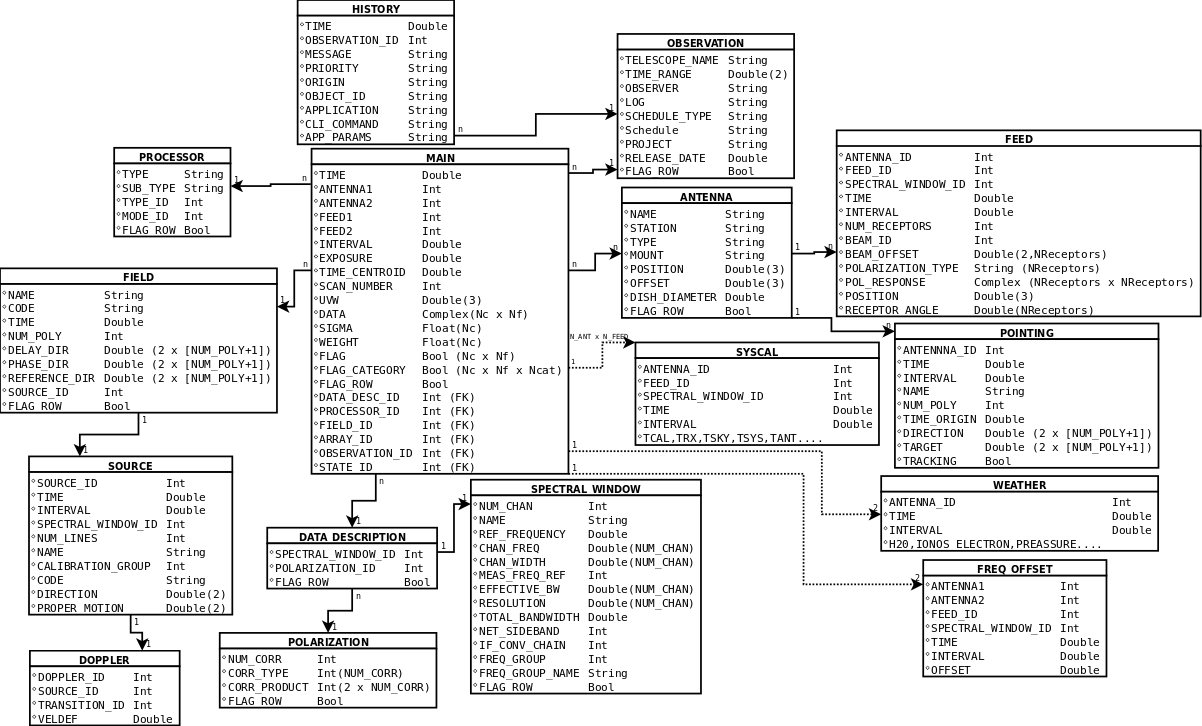
\includegraphics[height=0.35\textheight,width=0.8\textwidth]{images/ms_relations.png}
  \caption[Measurement Set schema]{This diagram depicts the standard layout of a Measurement Set database. Only some of the optional fields
  are included in this diagram, for instance the MAIN table may have multiple data columns and per channel weights. Only the most important
  relations are shown in this diagram. Data can be queried using a SQL-like language known as TaQL.}
  \label{FIG_MS_RELATIONS}
 \end{mdframed}
\end{figure}

Each row in the MAIN table contains measurements for a particular spectral band and may contain multiple correlations per spectral channel. Each
row contains $N_\text{channel}\times N_\text{correlation}$ measurements. The rows is not necessarily 
ordered by either baseline, time or antenna IDs by default and in total the Measurement Set MAIN table
will contain $N_\text{baseline}\times \frac{\tau_\text{observed time}}{\tau_\text{integration length}}$ rows, including autocorrelated antennas. It is worth noting 
that during flagging and calibration some rows may be deleted from the Measurement Set.

Bullseye is designed to handle observations split into multiple Measurement Sets as input. When more than one Measurement Set is specified as input it is assumed that
the two measurement sets contain observations of the same set of fields and that all the metadata remains the same between the two databases.

\subsection{The Flexible Image Transport System}
Our facet imager has to output a series of image cubes, one per facet. Each facet cube is a 3-dimensional array containing continuum images at multiple 
frequency bins, where several channels in the measurement set may be averaged into each of these slices. The Flexible Image Transport System (FITS) \cite{pence2010definition} 
format has been the defacto standard for data sharing between observatories. A FITS file can be used to store an N-dimensional data cube where N can range between 1 and 999 and is
structured as a series of Header Data unit blocks, each 2880 bytes in size. Each header contains a series of 80 character key-value pairs that 
describe the coordinates of each of the axes, along with projection and transformation information.

Since the primary goal of our imager is to make facet images, we choose to use the orthogonal projection coordinate system for the l and m coordinates. The orthogonal
projection results in coordinate distortions away from the projection pole. Since the primary goal of our imager to create narrow field facet images using this projection is
justified.

\section{Parallelizing data precomputation and resampling}
\subsection{Disk I/O vs. compute}
Although it is important to consider the computational costs involved with the resampling operation it is also necessary to take the latencies of loading
and preprocessing into account. When performing narrow field imaging, indeed the costs of disk I/O alone can amount to a significant portion of the run time.
The effect is less severe when performing faceting and w-projection. In order to mitigate this latency we opt to split the data into many pieces, making it possible
to load the next chunk into buffers while still imaging data already loaded and preprocessed as illustrated in Figure~\ref{fig_async_compute}.

\begin{figure}[ht!]
 \begin{mdframed}
 \centering
  \begin{tikzpicture}[node distance=4.5cm]
    \node (start) [start] {};
    \node (load) [draw,trapezium,trapezium left angle=70,trapezium right angle=-70,maximum width=1cm,right of=start] {%
							      \begin{varwidth}{10em}
								Read data from MS
							      \end{varwidth}};
    \node (preprocess) [process, right of=load] {Preprocess};
    \node (image) [process, right of=preprocess] {Image};
    \node (lastchunk) [decision, below of=preprocess] {Last chunk?};
    \node (stop) [stop, right of=lastchunk] {};
    
    \draw [rarrow] (start) -- (load);
    \draw [rarrow] (load) -- (preprocess);
    \draw [rarrow] (preprocess) -- (lastchunk);
    \draw [dashed,rarrow] (preprocess) -- (image) node [midway, above, sloped] (async_node) {Async};
    \draw [rarrow] (lastchunk) -- (load) node [midway, above, sloped] (no_node) {No};
    \draw [rarrow] (lastchunk) -- (stop) node [midway, above, sloped] (yes_node) {Yes};
  \end{tikzpicture}
 \caption[Aynchronous compute]{Asynchronous compute while data is buffered. The imaging algorithms are invoked on a background thread while the main 
 program thread continues to buffer in the next chunk of data. We use a thread barrier mechanism to ensure that the previous round of imaging has completed before starting
 to image the next chunk.}
 \label{fig_async_compute}
 \end{mdframed}
\end{figure}

When performing widefield imaging with a large number of facets and/or w-projection with filters of large support the latency involved with disk
I/O is effectively hidden and the runtime is bound by the compute time. All but the cost of loading the first chunk of data is hidden by this strategy.

\subsection{The CPU-based resampling algorithm}
The requirement of creating a field containing multiple facets provides a course-grained approach to parallelizing the resampling process,
without the need for synchronization and locks. This parallelization strategy works well when there are at least as many facets as CPU cores 
on the system, especially when the number of facets is close to a multiple of the number of CPU cores, balancing the workload between cores. The
parallelization is implemented using the lightweight OpenMP framework of macros.

The resampling algorithm should cater for gridding multiple correlations and enabling faceting and w-projection-based resampling when required.
To achieve this efficiently and with maximum reuse of code the resampling algorithm is implemented using a set of traits and policy C++ templates.
Algorithm~\ref{ALG_GRIDDING_CPU} is simplified pseudo code, but explains the core resampling steps on a CPU.

\begin{algorithm}
 \begin{algorithmic}
  \STATE {Allocate a complex grid $g$ of size $n \times m$ pixels for each facet and cube slice}
  \STATE {Assume $N_\text{rows}$ of complex visibilities, uvw coordinates, weights and flags is read from database}
  \STATE {Let $c$ be a padded complex filter with $N_\text{planes}$ w-layers}
  \STATE {By scaling the uv tracks the IFFT is scaled to the desired field of view (simularity theorem):}
  \STATE {Let $u_\text{scale} = $ ARCSEC\_TO\_RADIANS($n\times cellsize_l$)}
  \STATE {Let $v_\text{scale} = $ ARCSEC\_TO\_RADIANS($m\times cellsize_m$)}
  \FOR {(in parallel) $f \in [0...N_\text{facets})$}
    \FOR {$r \in [0...N_\text{rows})$}
      \IF {$field[r]$ not being gridded \OR $rowFlagged[r]$}
	  \STATE {continue}
      \ENDIF
      \FOR {$q \in [0...N_\text{channels})$}
	\IF {$channelFlagged[r,q]$}
	  \STATE {continue}
	\ENDIF
	\FOR {$x \in [0...N_\text{cross correlations})$}
	  \STATE {Let cube\_slice be the index of the grid frequency $spw[r]\times N_\text{chan} + q$ is to be accumulated to}
	  \STATE {Let $u,v,w = \frac{u[r]\times u_\text{scale}}{\text{wavelength}[q]}$,$\frac{v[r]\times v_\text{scale}}{\text{wavelength}[q]},\frac{w[r]}{\text{wavelength}[q]}$}
	  \STATE {First apply facet phase steer to original scaled uvw coordinates and orthogonal lmn coordinates:}
	  \STATE {Let $p_f=\exp{(2\pi i/\lambda[u(l_i-l_0)+v(m_i-m_0)+w(n_i-n_0)])}$}
	  \IF {doing polyhedron faceting}
	    \STATE {Tilt the facet by rotating the uv plane:}
	    \STATE {Let $uvw'$ be a set of rotated $uvw$ coordinates, applying $R(\alpha_i,\delta_i)R^{T}(\alpha_0,\delta_0)$}
	  \ENDIF
	  \STATE {Let $u'_\text{int},v'_\text{int}$ be the rounded (to nearest integer) $u',v'$}
	  \STATE {Let $u'_\text{frac},v'_\text{frac} = -u'+u'_\text{int},-v'+v'_\text{int}$}
	  \STATE{Let $vis = vis[r,q,x]$}
	  \STATE{Instead of storing convolution kernels for negative w grid the complex conjugates of the baselines:}
	  \IF {$w' < 0$}
	    \STATE {Let $vis = $conjugate($vis$)}
	    \STATE {Let $u',v',w' \times = -1$}
	  \ENDIF
	  \STATE{Assuming linear spacing between sampled w layers:}
	  \STATE{Let $w_\text{plane} = \text{round}(w'/w_{max}\times(N_\text{planes}-1))$}
	  \IF {$u'_\text{int},v'_\text{int} \pm c_\text{half support}$ within grid boundaries}
	    \FOR {$v_\text{tap} \in [-c_\text{half support}...c_\text{half support}]$}
	      \FOR {$u_\text{tap} \in [-c_\text{half support}...c_\text{half support}]$} 
		\STATE {Let $c_\text{weight} = c[(u_\text{tap} + c_\text{half support} + u'_\text{frac} + 1)) \times c_\text{oversample},(v_\text{tap} + c_\text{half support} + v'_\text{frac} + 1)) \times c_\text{oversample},w_\text{plane}]$}
		\STATE {Let $g[u'_\text{int} + u_\text{tap} + \frac{n}{2},v'_\text{int} + v_\text{tap} + \frac{m}{2},\text{cube\_slice}] += vis \times p_f \times c_\text{weight}$}
	      \ENDFOR
	    \ENDFOR
	  \ENDIF
	\ENDFOR
      \ENDFOR
    \ENDFOR
  \ENDFOR
 \end{algorithmic}
 \caption{CPU facet-based convolutional resampling}
 \label{ALG_GRIDDING_CPU}
\end{algorithm}

If the channels all contribute to different grids in the cube it can provide another avenue of parallelization. However, we assumed that the input data is used to
construct a set of continuuim images per cube. As such the wavelengths used in the algorithm to scale the uv tracks are those provided in the measurement set and are in the topocentric
frame of reference. As such the imager should not be used to create spectral line images where it is essential that the frame of reference is stable during the course of the observation.
Such observations require that the uvw coordinates are corrected for the dopler-shifts introduced by the Earth's rotation around its axis and around the sun. This is an expensive time-dependent
correction and provided by the casacore libraries. The correction is not used at present.

The innermost loops computes and writes values to consecutive grid locations and is responsible for the quadratic scaling factor that makes w-projection-based resampling such an expensive operation. 
This opens up the opportunity to further parallelization on CPUs that support vector processing operations through SSE and AVX. The GCC compiler suite does not automatically vectorize the code in the inner-most 
loop during automatic optimization due to its depth. We therefore had to vectorize the code for the innermost loop by hand for the seperate cases of gridding 1, 2 and 4 cross correlations. Vectorization will have
the greatest impact when performing w-projection and therefore only this use case was vectorized. Instead of writing separate SSE and AVX versions of the code we decided to only support modern processors that include the 
AVX instruction set. Older processors can be targeted during compile time by turning off the vectorizated code.

The vectorized instructions load the original values from consecutive grid positions, parallelizes the complex multiplications and additions, finally storing the values back to the grid positions in memory. It is important to
realize that both the optimized load and store instructions require that the index of the first float be aligned to 16-byte boundaries. Since the rounded u,v coordinates can fall anywhere on the grid this alignment cannot be guarenteed,
even if the grid memory is aligned when allocated. It is therefore necessary to use the unoptimized load and store operations which will hamper performance to some degree.

\subsection{The GPU-based resampling algorithm}
The GPU work distribution strategy is more complicated than that of the CPU. A GPU co-processor has thousands of processing cores and it is therefore imparitive to spawn enough threads to fully
occupy all the cores the GPU. Furthermore the computational throughput on these GPUs are more than 60x faster than access to global memory, highlighting the importantance to limit the total global 
memory accesses made by the gridding algorithm. The approach we choose for our implementation is a distribution strategy first
suggested by John Romein \cite{romein2012efficient}.

The strategy exploits the spacial locality between consecutive measurements made by the same baseline. As long as the integration time
between consecutive measurements are short the measurements should fall on the same grid points. The strategy accumulates the values that fall 
within the same grid cell in a register before writing the value out to global memory when the uv track moves onto the next grid point.
Each thread is assigned one tap in the support area of the convolution filter and one of each of these groups are assigned to a baseline.
Many baselines can therefore be gridded in parallel, assuming the write accesses to global memory are atomic to ensure the resulting race conditions
between two or more baseline thread groups are mitigated.

The approach assumes of course that the data is grouped per baseline and then ordered by time.
The data within a measurement set is not generally ordered like this and it is necessary to repack the 
data as part of the loading and preprocessing step, as indicated in Figure~\ref{fig_gpu_preprocess}.
\begin{figure}[ht!]
 \begin{mdframed}
 \centering
  \begin{tikzpicture}[node distance=4.5cm]
    \node (start) [start] {};
    \node (data) [draw,trapezium,trapezium left angle=70,trapezium right angle=-70,maximum width=1cm,right of=start] {%
							      \begin{varwidth}{10em}
								Read data from MS
							      \end{varwidth}};
    \node (sort) [process, right of=data] {Sort by time};
    \node (count) [process, right of=sort] {Count measurements per baseline};
    \node (prescan) [process, below of=count] {Compute starting indexes};
    \node (image) [process, left of=prescan] {Copy to GPU and image};
    \node (stop) [stop, left of=image] {};
    
    \draw [rarrow] (start) -- (data);
    \draw [rarrow] (data) -- (sort);
    \draw [rarrow] (sort) -- (count);
    \draw [rarrow] (count) -- (prescan);
    \draw [rarrow] (prescan) -- (image);
    \draw [rarrow] (image) -- (stop);
  \end{tikzpicture}
 \caption[GPU preprocessing workflow]{The preprocessing workflow necessary for gridding using
 Romein's distribution strategy.}
 \label{fig_gpu_preprocess}
 \end{mdframed}
\end{figure}

After reordering the entire measurement set by time it is important to repack the data by baseline. 
Not all baselines have the same number of timesteps (some may have been split out of the measurement 
set during the flagging and calibration process), requiring that a variable-length array is allocated
per baseline. Such a variable length array of arrays is not easy to transfer onto the GPU and we instead
opt to flatten this array into a one dimensional structure, storing the positions of the first time step
of each baseline as a separate array. Such an approach require that a single pass over the data counting 
the number of timesteps per baseline. A running accumulation (or \textit{prefix scan}) of these counts
is then computed, yielding the starting indexes of the baseline subarrays. The baseline index is not
stored directly in a measurement set: only the id's of the antennae are stored. The unique identifier
for each of the baselines are given by the following quadratic series:
\begin{equation}
 i_{a_2-a_1} = (-S^2 + 2\times S\times N_\text{antennae} + S) / 2 + |a_1 - a_2|, S := \min(a_1,a_2)
\end{equation}
It is important to note that the measurement set only stores unique measurements and not their conjugate 
counterparts, and hence there are only (at maximum) $\frac{N_\text{antennae}(N_\text{antennae} - 1)}{2} + N_\text{antennae}$
measurements per timestep, including the autocorrelated measurements of each of the antennae.

The prefix scan operator (for the normal binary-associative addition operator) is defined as:
\begin{equation}
 \text{prescan}(C)[i] = 
			\begin{cases}
			  0 & i = 0 \\
			  \sum_{k=0}^{i-1}{C[k]} & i > 0 \\
			\end{cases}
\end{equation}

It is therefore necessary to allocate an array to store the baseline counts with $N_\text{baselines} + 1$, setting the last element to zero,
in order to store the starting indicies of all the baselines and implicitly store the number of elements contained in the sub-array of the last
baseline.

Once the starting indexes are computed the repacked arrays are transferred onto the GPU and when completed the gridding gpu kernel is 
launched asyncronously and the next set of uv coordinates and visibilities are read, and the required preprocessing started, similar 
to the CPU implementation. It is also important to mention that the correlations not being gridded is stripped out of the visibility 
array before transfer, to reduce the transfer time.

The resampling approach taken on GPUs is stated in Algorithm~\ref{ALG_GRIDDING_GPU}. The kernel, as stated in the algorithm, is dispatched to 
$c_\text{full support}\times c_\text{full support}\times N_\text{baselines}\times N_\text{facets}$ threads when launched and broken
into blocks of threads a multiple of the cuda device \textit{warp length} in size. Given enough registers for each thread this approach
should achieve high occupancy on the GPU. It may be necessary to adjust the maximum number of registers per thread through command line 
arguments to the compiler to ensure that the maximum number of registers available per Streaming Multiprocessor is not exceeded, depending on
the targeted device.

\begin{algorithm}
 \begin{algorithmic}
  \STATE {Allocate a complex grid $g$ of size $n \times m$ pixels for each facet and cube slice}
  \STATE {Assume $N_\text{rows}$ of complex visibilities, uvw coordinates, weights and flags is read and transfered to GPU}
  \STATE {Let $c$ be a padded complex filter with $N_\text{planes}$ w-layers}
  \STATE {By scaling the uv tracks the IFFT is scaled to the desired field of view (simularity theorem):}
  \STATE {Let $u_\text{scale} = $ ARCSEC\_TO\_RADIANS($n\times cellsize_l$)}
  \STATE {Let $v_\text{scale} = $ ARCSEC\_TO\_RADIANS($m\times cellsize_m$)}
  \STATE {Compute $u_\text{tap},v_\text{tap},b_i,f_i$ from the thread index}
  \STATE {Let $s$ be the computed starting indexes (computed prior to launch)}
  \STATE {Let $u_\text{prev},v_\text{prev}$ be the previous u,v grid coordinates initially 0}
  \STATE {Let $vis_x = 0+0i$ be the visibility accumulators for $x = 1,2 \text{ or } 4$ correlations}
  \FOR {$q \in [0...N_\text{channels})$}
    \STATE {Let cube\_slice be the index of the grid frequency $spw[r]\times N_\text{chan} + q$ is to be accumulated to}
    \FOR {$r \in [s[b_i]...s[b_i + 1])$}
      \IF {$field[r]$ not being gridded \OR $rowFlagged[r]$ \OR $channelFlagged[r,q]$}
	\STATE {continue}
      \ENDIF
      \STATE {Let $u,v,w = \frac{u[r]\times u_\text{scale}}{\text{wavelength}[q]}$,$\frac{v[r]\times v_\text{scale}}{\text{wavelength}[q]},\frac{w[r]}{\text{wavelength}[q]}$}
      \STATE {First apply facet phase steer to original scaled uvw coordinates and orthogonal lmn coordinates:}
      \STATE {Let $p_f=\exp{(2\pi i/\lambda[u(l_i-l_0)+v(m_i-m_0)+w(n_i-n_0)])}$}
      \IF {doing polyhedron faceting}
	\STATE {Tilt the facet by rotating the uv plane:}
	\STATE {Let $uvw'$ be a set of rotated $uvw$ coordinates, applying $R(\alpha_i,\delta_i)R^{T}(\alpha_0,\delta_0)$}
      \ENDIF
      \STATE {Let $u'_\text{int},v'_\text{int}$ be the rounded (to nearest integer) $u',v'$}
      \STATE {Let $u'_\text{frac},v'_\text{frac} = -u'+u'_\text{int},-v'+v'_\text{int}$}
      \FOR {$x \in [0...N_\text{cross correlations})$}	  	  
	  \STATE{Let $vis = vis[r,q,x]$}
	  \STATE{Instead of storing convolution kernels for negative w grid the complex conjugates of the baselines:}
	  \IF {$w' < 0$}
	    \STATE {Let $vis = $conjugate($vis$)}
	    \STATE {Let $u',v',w' \times = -1$}
	  \ENDIF
	  \STATE{Assuming linear spacing between sampled w layers:}
	  \STATE{Let $w_\text{plane} = \text{round}(w'/w_{max}\times(N_\text{planes}-1))$}
	  \IF {$u_\text{prev} \neq u_\text{int}$ \OR $v_\text{prev} \neq v_\text{int}$}
	    \IF {$u'_\text{int},v'_\text{int} \pm c_\text{half support}$ within grid boundaries}
	      \STATE {Let $g[u'_\text{prev} + u_\text{tap} + \frac{n}{2},v'_\text{prev} + v_\text{tap} + \frac{m}{2},\text{cube\_slice}] += vis_x$}
	    \ENDIF
	    \STATE {Let $u_\text{prev} = u_\text{int}, v_\text{prev} = v_\text{int}, vis_x = 0+0i$}
	 \ENDIF
	 \STATE {Let $c_\text{weight} = c[(u_\text{tap} + c_\text{half support} + u'_\text{frac} + 1)) \times c_\text{oversample},(v_\text{tap} + c_\text{half support} + v'_\text{frac} + 1)) \times c_\text{oversample},w_\text{plane}]$}
	 \STATE {Let $vis_x += vis \times p_f \times c_\text{weight}$}
      \ENDFOR % x
    \ENDFOR % r 
    \IF {$u'_\text{int},v'_\text{int} \pm c_\text{half support}$ within grid boundaries}
	\STATE {Let $g[u'_\text{prev} + u_\text{tap} + \frac{n}{2},v'_\text{prev} + v_\text{tap} + \frac{m}{2},\text{cube\_slice}] += vis_x$}
    \ENDIF
    \STATE {Let $u_\text{prev} = u_\text{int}, v_\text{prev} = v_\text{int}, (\forall x \in [0...N_\text{cross correlations}-1))vis_x = 0+0i$}
  \ENDFOR % q
 \end{algorithmic}
 \caption{GPU facet-based convolutional resampling}
 \label{ALG_GRIDDING_GPU}
\end{algorithm}
\section{GPU filter caching option}
The GPU has several on- and off-chip memory types and caching mechanisms as already discussed. Due to the spacial locality of the convolution filter lookups it is advantageous to
store the filter values in a memory that is cached on chip. GPU texture memory is off-chip read-only memory, but 48 KB (Kepler architecture) is 
cached on-chip and is ideal for storing convolution kernels. 

When convolving with seperable filters like those used in narrow field imaging this is plenty. However, as we already pointed out
w-projection filters are not generally seperable filters. This results in high memory usage when the oversampling factor and number of w layers are 
increased. However, for the GPU implementation we assumed that w-projection will always be used in conjunction with faceting, since coplanar w-faceting
is the primary mechanism by which our imager removes the widefield effect. As we already shown w-projection filters are approximately seperable when 
imaging over narrow fields of view, and these filters have a much better chance to fit into texture cache. Our GPU w-projection implementation
assumes that the seperable filter implementation is accurate enough for the user and it is important that faceting always be enabled when imaging on 
the GPU.

We have provided an alternative cache-less implementation of the GPU imager for comparison and compatibility.
If the stack of filters are too big to fit into memory the caching code can be turned off at compile time. We have seen
a ~20\% drop in performance on compute 3.0 hardware with this option disabled.

\section{Precision}
During the course of an observation the gridding operation accumulates thousands of complex-valued visibilities into a set of grid bins. Since this operation
is done in finite precision the summation of such a large number of visibilities is prone to rounding error. Nicholas Higham \cite{higham1993accuracy} shows that
an upper bound for summation error is given by the following for any well-behaved summation method:
\begin{equation}
 |E_n| \leq (n-1)u\sum_{i=1}^{n}{|x_i|} + O(u^2), u := \frac{\beta}{2}\beta^{-\rho}
\end{equation}
Here $u$ is the machine epsilon and assumed to have $\beta=2$ and $\rho=24$ or $\rho=53$ for IEEE 754 single and double precision respectively (David Goldberg \cite{goldberg1991every}
gives a detailed discussion), and hence the $u^2$ term can be ignored.

The error scales with the number of terms as well as the magnitude of the terms. This is concerning because recent trends in interferometers have
seen a significant growth in the number of baselines and channels, and hence the number of visibilities being accumulated. Large arrays also require
convolution kernels with large support which will futher worsten the effects of total rounding error accross the grid. We have decided to provide 
a set of single and double precision gridding routines in order to test how this effects the accuracy of the synthesized images. Since the FFT preserves
the total energy between the spacial and frequency domains (Parseval's theorem) we expect the rounding error to be present in the brightness of sources in 
the reconstructed images. The difference between single and double precision synthesis for extended observations will be investigated in the results section.

The choice between single and double precision synthesis has a significant performance impact on GPUs where the number of double precision units are significantly
less than single precision units (1 to 3 in the case of Kepler generation GPUs). The performance impact will be determined experimentally in the results section.
\section{Faceting options}
Our imager supports both targeted and continuous faceting. In the instance of targeted faceting (demonstrated in Figure~\ref{FIG_TARGET_GUI}) the user specifies a set of coordinates 
for the facet centres, along with the size of the facet images to be created. In continuous faceting mode the user specifies the size of the facets along with the number of facets in
both l and m. The current implementation joins the facets at the facet edges, with no overlap. It is therefore necessary to pad each of the facet images to
reduce the remaining aliasing energy that is normally encountered right at the edge of the image (as discussed not all the energy is stopped due to filter roll off).

It is important to note that the \texttt{CRVALn} keywords for the l and m coordinates in each of the facet image cubes are the coordiantes of the original phase tracking centre $l_0,m_0$, even
if those coordinates fall outside the area of the facet images. This is necessary to ensure that the facets all share the same divergence in coordinates that follows from using the 
orthogonal (``SIN'') projection.

We have included a prototype graphical interface to demonstrate facet imaging, shown here in Figure~\ref{FIG_TARGETED_FACETING}. The prototype tool is implemented in Python and uses the GTK
framework. It calls directly on the command line interface of our imager.
\begin{figure}[ht!]
 \begin{mdframed}
  \centering
  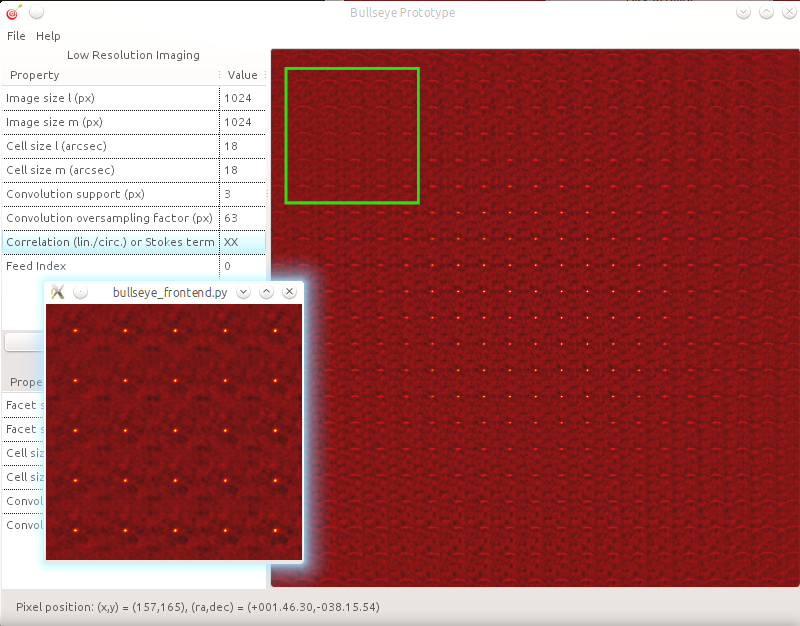
\includegraphics[width=0.75\textwidth]{images/targeted_faceting.png}
  \caption[Targeted faceting in action]{The result of faceting a narrow piece of sky that is far away from the phase tracking centre of the telescope. Here a simulated gridded sky pattern
  shows the widefield distortions of sources far away from the field centre. In the facet image of this area all the sources are corrected.}
  \label{FIG_TARGETED_FACETING}
 \end{mdframed}
\end{figure}

When constructing continuous images the user has the option to reproject and combine the individual facet images using the Montage \cite{jacob2004montage} suite of tasks after the facets have been
synthesized.

\section{Image normalization}
Each of the images are normalized by a counter that takes weights, flagged and visibilties that are not gridded into account:
\begin{equation}
 N = \sum_{k=0}^{M-1}{\sum_{u_\text{tap}=0}^{\text{full sup}}{\sum_{v_\text{tap}=0}^{\text{full sup}}{c[(u_\text{tap}+u[k]_\text{frac} + 1)\times c_\text{oversamp},(v_\text{tap}+v[k]_\text{frac} + 1)\times c_\text{oversamp}]}} W[k]\neg F[k]}
\end{equation}
Due to the linearity of the fourier transform this normalization can be applied per grid point or synthesized image pixel. On the GPU it is necessary to keep an extra register per thread and reduce
to a single value after gridding is completed.

It is also possible to normalize by the centre value of the point spread function, but this requires that the PSF always be synthesized. When a full deconvolution pipeline is added to the imager this step
can be changed.

\section{Validation and testing}
We used both simulated and real data to to test our imager. We chose to support the Measurement Set format because of its widespread use in radio astronomy. Thus far we have tested our imager only on real data generated
by the EVLA. Specifically we followed the calibration and flagging guidelines for the supernova remnant G55.7+3.4 observed by the EVLA in L-band. The guide is available at \url{https://casaguides.nrao.edu/index.php/EVLA_Wide-Band_Wide-Field_Imaging:_G55.7_3.4-CASA4.4}.
The observed field contains sources that had been identified as being distorted by the widefield effect. These sources are also bright enough to be clearly visible in the dirty images, making this dataset ideal for use in
testing our imager.

\begin{figure}[h!]
  \centering
 \begin{subfigure}[b]{0.49\textwidth}
    \centering
    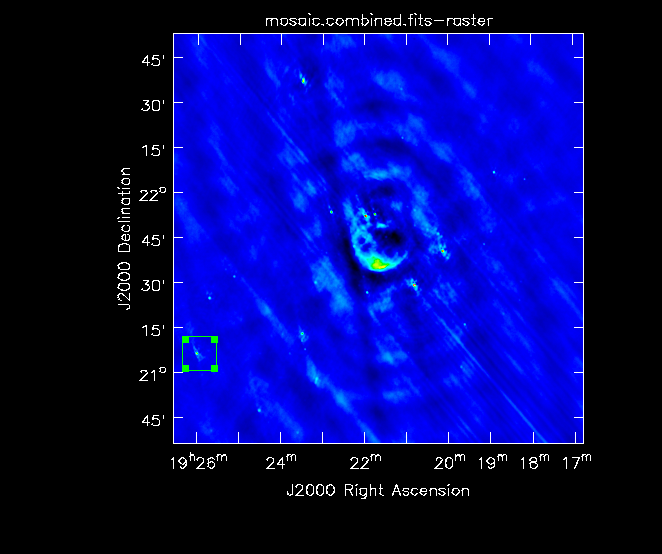
\includegraphics[width=\textwidth]{images/validation/mosaic.png}
    \caption{Mosaiced faceted image (2x2 facets, 1.2\% padding each). No additional w-projection.}
 \end{subfigure}
 \begin{subfigure}[b]{0.49\textwidth}
    \centering
    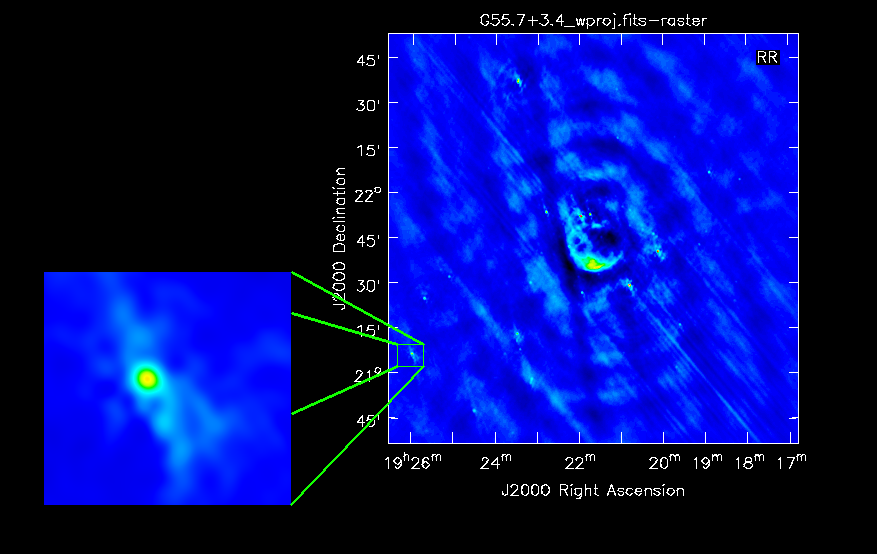
\includegraphics[width=\textwidth]{images/validation/wproj.png}
    \caption{W-projected image. No faceting.}
 \end{subfigure}
 \begin{subfigure}[b]{0.49\textwidth}
    \centering
    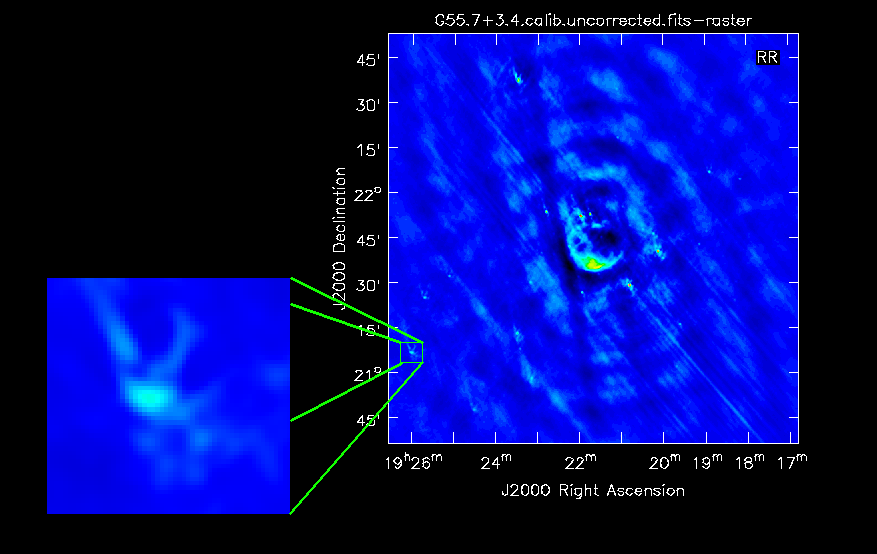
\includegraphics[width=\textwidth]{images/validation/uncorrected.png}
    \caption{Uncorrected image (normal narrow field imaging).}
 \end{subfigure}
 \begin{subfigure}[b]{0.49\textwidth}
    \centering
    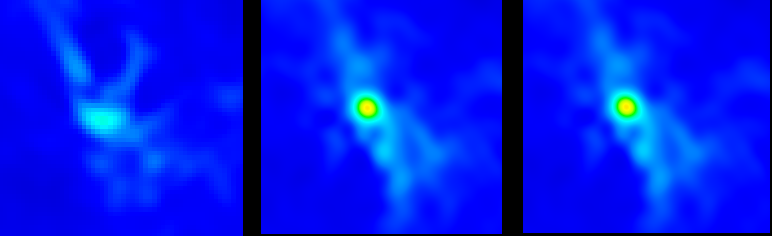
\includegraphics[width=\textwidth]{images/validation/corrections.png}
    \caption{Up close, from the left: the uncorrected source, the faceted source and 
    finally the w-projected source}
 \end{subfigure}
 \caption[Supernova reminant G55.7+3.4]{In this field there is a clear widefield distorition near
 right assention $19h26m$, declination $21^\circ7'$. Both the faceting and w-projection
 implementations corrects the distortion as expected. The w-projected image here uses no faceting
 and simularly the faceting was done by enabling only a first order approximation for w and disabling
 w-projection.}
 \label{FIG_SUPERNOVA}
\end{figure}